%% =============================================================================
%%  Material suplementario del articulo de optimizacion (IEEEtran, journal). Compilar con pdfLaTeX.
%%  Las tablas tabla_s_*.tex las genera codigo/gen_tablas_opt.py desde resultados/opt/*.json.
%% =============================================================================
\documentclass[journal]{IEEEtran}
\usepackage[utf8]{inputenc}
\usepackage[T1]{fontenc}
\usepackage[spanish,es-tabla,es-nodecimaldot]{babel}
\addto\captionsspanish{\renewcommand{\figurename}{Fig.}}
\usepackage{cite}
\usepackage{amsmath,amssymb}
\usepackage{graphicx}
\usepackage{booktabs}
\usepackage[table]{xcolor}
\usepackage{array}
\usepackage{url}
\graphicspath{{figures/}}
% Generado por gen_tablas_opt.py (no editar a mano)
\newcommand{\DelayOfFijo}{13.81}
\newcommand{\DelayOfAct}{10.89}
\newcommand{\DelayOfActAf}{9.63}
\newcommand{\DelayOfMax}{17.44}
\newcommand{\DelayOfPap}{10.95}
\newcommand{\DelayOfPapAf}{9.67}
\newcommand{\DelayOfMdp}{9.35}
\newcommand{\DelayOfFlc}{7.91}
\newcommand{\DelayOfFlcC}{9.97}
\newcommand{\DelayOfMlp}{8.09}
\newcommand{\DelayOfMlpC}{9.46}
\newcommand{\DelayNvFijo}{13.00}
\newcommand{\DelayNvAct}{10.55}
\newcommand{\DelayNvActAf}{9.17}
\newcommand{\DelayNvMax}{16.55}
\newcommand{\DelayNvPap}{10.40}
\newcommand{\DelayNvPapAf}{9.30}
\newcommand{\DelayNvMdp}{8.77}
\newcommand{\DelayNvFlc}{7.40}
\newcommand{\DelayNvFlcC}{9.37}
\newcommand{\DelayNvMlp}{7.53}
\newcommand{\DelayNvMlpC}{8.95}
\newcommand{\DelayVaFijo}{12.29}
\newcommand{\DelayVaAct}{9.23}
\newcommand{\DelayVaActAf}{8.07}
\newcommand{\DelayVaMax}{19.00}
\newcommand{\DelayVaPap}{8.65}
\newcommand{\DelayVaPapAf}{8.06}
\newcommand{\DelayVaMdp}{7.94}
\newcommand{\DelayVaFlc}{6.07}
\newcommand{\DelayVaFlcC}{8.41}
\newcommand{\DelayVaMlp}{6.24}
\newcommand{\DelayVaMlpC}{8.05}
\newcommand{\DelaySaFijo}{40.67}
\newcommand{\DelaySaAct}{54.06}
\newcommand{\DelaySaActAf}{24.13}
\newcommand{\DelaySaMax}{152.25}
\newcommand{\DelaySaPap}{105.87}
\newcommand{\DelaySaPapAf}{58.11}
\newcommand{\DelaySaFlc}{24.29}
\newcommand{\DelaySaFlcC}{25.74}
\newcommand{\DelaySaMlp}{25.10}
\newcommand{\DelaySaMlpC}{24.29}
\newcommand{\RedFijo}{$-$26.1}
\newcommand{\RedAct}{0.6}
\newcommand{\RedActAf}{12.1}
\newcommand{\RedMax}{$-$59.3}
\newcommand{\RedPapAf}{11.7}
\newcommand{\RedMdp}{14.7}
\newcommand{\RedFlc}{27.8}
\newcommand{\RedFlcC}{9.0}
\newcommand{\RedMlp}{26.2}
\newcommand{\RedMlpC}{13.6}
\newcommand{\RedPapOf}{27.8}
\newcommand{\RedActAfOf}{17.8}
\newcommand{\RedPapNv}{28.8}
\newcommand{\RedActAfNv}{19.3}
\newcommand{\RedPapVa}{29.8}
\newcommand{\RedActAfVa}{24.7}
\newcommand{\RedPapSa}{77.1}
\newcommand{\RedActAfSa}{$-$0.7}
\newcommand{\ParMediaPap}{28.2}
\newcommand{\ParMejorPap}{16}
\newcommand{\ParPeorPap}{0}
\newcommand{\ParMinPap}{19.5}
\newcommand{\ParMaxPap}{49.3}
\newcommand{\ParMediaActAf}{22.0}
\newcommand{\ParMejorActAf}{16}
\newcommand{\ParPeorActAf}{0}
\newcommand{\ParMinActAf}{2.9}
\newcommand{\ParMaxActAf}{46.5}
\newcommand{\ParMediaAct}{31.3}
\newcommand{\ParMejorAct}{16}
\newcommand{\ParPeorAct}{0}
\newcommand{\ParMinAct}{11.4}
\newcommand{\ParMaxAct}{56.8}
\newcommand{\ParMediaFijo}{44.1}
\newcommand{\ParMejorFijo}{16}
\newcommand{\ParPeorFijo}{0}
\newcommand{\ParMinFijo}{39.2}
\newcommand{\ParMaxFijo}{61.2}
\newcommand{\ParMediaMdp}{19.2}
\newcommand{\ParMejorMdp}{16}
\newcommand{\ParPeorMdp}{0}
\newcommand{\ParMinMdp}{2.7}
\newcommand{\ParMaxMdp}{43.5}
\newcommand{\DelayOfFijos}{8.44}
\newcommand{\DelayNvFijos}{7.88}
\newcommand{\DelayVaFijos}{6.56}
\newcommand{\DelaySaFijos}{24.80}
\newcommand{\RedActFijos}{12.3}
\newcommand{\RedPapFijos}{22.9}
\newcommand{\DelayOfReglas}{8.47}
\newcommand{\DelayNvReglas}{7.93}
\newcommand{\DelayVaReglas}{6.55}
\newcommand{\DelaySaReglas}{25.00}
\newcommand{\RedActReglas}{12.0}
\newcommand{\RedPapReglas}{22.6}
\newcommand{\DelayOfGSiete}{8.60}
\newcommand{\DelayNvGSiete}{8.14}
\newcommand{\DelayVaGSiete}{6.85}
\newcommand{\DelaySaGSiete}{25.15}
\newcommand{\RedActGSiete}{10.6}
\newcommand{\RedPapGSiete}{21.4}
\newcommand{\DelayOfGCinco}{8.21}
\newcommand{\DelayNvGCinco}{7.75}
\newcommand{\DelayVaGCinco}{6.41}
\newcommand{\DelaySaGCinco}{25.16}
\newcommand{\RedActGCinco}{14.8}
\newcommand{\RedPapGCinco}{25.1}
\newcommand{\DelayOfGCuatro}{8.04}
\newcommand{\DelayNvGCuatro}{7.58}
\newcommand{\DelayVaGCuatro}{6.20}
\newcommand{\DelaySaGCuatro}{24.38}
\newcommand{\RedActGCuatro}{16.5}
\newcommand{\RedPapGCuatro}{26.6}
\newcommand{\DelayOfSemCero}{8.00}
\newcommand{\DelayNvSemCero}{7.51}
\newcommand{\DelayVaSemCero}{6.21}
\newcommand{\DelaySaSemCero}{24.79}
\newcommand{\RedActSemCero}{16.9}
\newcommand{\RedPapSemCero}{26.9}
\newcommand{\DelayOfSemUno}{8.04}
\newcommand{\DelayNvSemUno}{7.49}
\newcommand{\DelayVaSemUno}{6.24}
\newcommand{\DelaySaSemUno}{24.63}
\newcommand{\RedActSemUno}{16.5}
\newcommand{\RedPapSemUno}{26.6}
\newcommand{\DelayOfSemDos}{7.91}
\newcommand{\DelayNvSemDos}{7.40}
\newcommand{\DelayVaSemDos}{6.07}
\newcommand{\DelaySaSemDos}{24.29}
\newcommand{\RedActSemDos}{17.8}
\newcommand{\RedPapSemDos}{27.8}
\newcommand{\DelayOfLinC}{9.53}
\newcommand{\DelayNvLinC}{8.97}
\newcommand{\DelayVaLinC}{8.10}
\newcommand{\DelaySaLinC}{25.11}
\newcommand{\RedActLinC}{1.0}
\newcommand{\RedPapLinC}{13.0}
\newcommand{\RedActFijo}{$-$43.4}
\newcommand{\RedActAct}{$-$13.1}
\newcommand{\RedActMax}{$-$81.2}
\newcommand{\RedActPap}{$-$13.8}
\newcommand{\RedActPapAf}{$-$0.4}
\newcommand{\RedActMdp}{2.9}
\newcommand{\RedActFlc}{17.8}
\newcommand{\RedActFlcC}{$-$3.5}
\newcommand{\RedActMlp}{16.0}
\newcommand{\RedActMlpC}{1.7}
\newcommand{\ResDifOf}{0.2}
\newcommand{\ResDifOfMax}{2.1}
\newcommand{\ResDifSa}{4.1}
\newcommand{\ResDifSaMax}{13.9}
\newcommand{\PdMaxDif}{0.7}

\newcommand{\fuente}[1]{\par\vspace{3pt}\noindent{\scriptsize\textit{Fuente:} #1\par}}
\renewcommand{\thetable}{S\arabic{table}}
\renewcommand{\thefigure}{S\arabic{figure}}
\newcommand{\qbar}{\bar{q}}
\newcommand{\FLC}{FLC-O}

\begin{document}
\title{Material suplementario: mejora de un controlador de semáforos de lógica difusa para una intersección aislada}
\author{Raul Nolberto Quispe Saya and Kevin Luis Valero Ccacya}
\markboth{Quispe Saya y Valero Ccacya: Material suplementario}{Quispe Saya y Valero Ccacya: Material suplementario}
\maketitle

\section{Alcance}
Este documento reúne los detalles del artículo principal que no caben en él: los hiperparámetros del entrenamiento, la verificación del simulador vectorizado, la cota por programación dinámica, los resultados completos del conjunto oficial, la sensibilidad a la semilla de entrenamiento y la forma de reproducir cada cifra. Las ecuaciones y secciones citadas son las del artículo principal.

\section{Entrenamiento}
\label{sec:s-entrena}
\begin{table}[t]
\centering
\caption{Configuración del entrenamiento con CMA-ES}
\label{tab:hiper}
\scriptsize
\begin{tabular}{@{}p{0.42\columnwidth}p{0.5\columnwidth}@{}}
\toprule
Elemento & Valor \\
\midrule
Algoritmo & $(\mu/\mu_w,\lambda)$-CMA-ES con pesos logarítmicos, CSA, actualización de rango uno y de rango $\mu$ \cite{Hansen2016}; implementación propia (\texttt{opt\_es.py}) \\
Población $\lambda$ y padres $\mu$ & $\lambda=4+\lfloor 3\ln n\rfloor$ ($n$ = número de parámetros), $\mu=\lfloor\lambda/2\rfloor$ \\
Paso inicial $\sigma_0$ & 0.3 (0.15 para Pappis y Mamdani afinado) \\
Generaciones & 120 a 200 según el modelo; punto de control cada 10 \\
Escenarios de entrenamiento & $N=64$ pares $(\qbar_1,\qbar_2)$ sorteados con $180\le$ cada brazo y suma de 540 a 3300\,veh/h; semillas de llegadas 100000 a 100063; 3600\,s \\
Escenarios de validación & 64 pares sorteados con otra semilla; llegadas 200000 a 200063; 7200\,s \\
Normalización del objetivo & retardo del actuado afinado en el mismo escenario (objetivo $J(\theta)$ del artículo, Sec.~VI-D) \\
Evaluación en paralelo & 4 procesos (\texttt{multiprocessing}, \texttt{fork}) \\
Verde máximo & 57\,s (Pappis y Mamdani); 90\,s (modelos entrenados con rango ampliado) \\
\bottomrule
\end{tabular}
\fuente{\texttt{codigo/opt\_es.py}, \texttt{codigo/opt\_entrenar\_modelo.py} y \texttt{codigo/opt\_entrenar.py}.}
\end{table}

\begin{figure}[t]
\centering
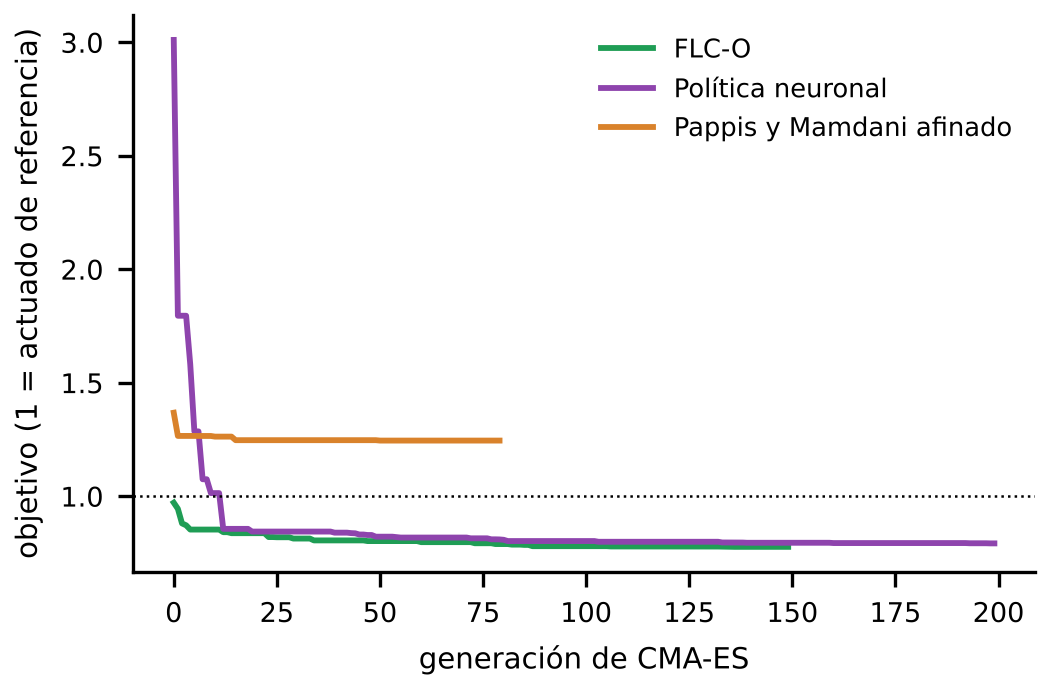
\includegraphics[width=\columnwidth]{fig_opt_aprendizaje.png}
\caption{Mejor valor del objetivo $J(\theta)$ por generación para los modelos finales (1: igual al actuado de referencia).}
\label{fig:s-aprendizaje}
\end{figure}

\section{Referencias afinadas}
\label{sec:s-ref}
El actuado y la presión máxima se afinaron con los mismos 64 escenarios de entrenamiento que los controladores aprendidos y dentro del mismo rango de verde mínimo (de 3 a 7\,s) y con verde máximo de a lo sumo 90\,s. La rejilla del actuado fue hueco de 1 a 3\,s, verde mínimo de 3 a 7\,s y máximo de 57, 80 y 90\,s (45 configuraciones); resultó hueco de 1\,s, mínimo de 3\,s y máximo de 90\,s. La de la presión máxima fue margen de 0, 1, 2, 3, 5, 8, 12 y 16 vehículos, mínimo de 3, 4, 5 y 7\,s y máximo de 57, 80 y 90\,s; resultó margen de 12 vehículos, mínimo de 4\,s y máximo de 57\,s. Una rejilla anterior, con verde mínimo de 5 a 10\,s y máximo de 57 a 120\,s (\texttt{resultados/opt/actuado\_afinado\_v1.json}), daba un actuado 5\,\% más lento: restringir el verde mínimo a 5\,s o más habría favorecido al controlador propuesto, y por eso se amplió. Los parámetros están en \texttt{resultados/opt/actuado\_afinado.json} y \texttt{resultados/opt/maxpressure\_afinado.json}.

\section{Verificación del simulador vectorizado}
\label{sec:s-equiv}
La prueba \texttt{test\_sim\_batch.py} (parte de las comprobaciones de \texttt{ejecutar\_pruebas.py}) simula 8 escenarios de 2400\,s con el simulador de referencia (\texttt{traffic\_model.py}) y con el vectorizado, y compara el retardo con las dos convenciones: con residuo y solo de los vehículos servidos.

\begin{table}[t]
\centering
\caption{Equivalencia entre el simulador vectorizado y el de referencia (8 escenarios)}
\label{tab:equiv}
\scriptsize
\begin{tabular}{@{}lr@{}}
\toprule
Controlador & Diferencia máxima (s/veh) \\
\midrule
Ciclo fijo de Webster (entero más próximo) & 0 \\
Ciclo fijo de Webster (reparto exacto) & 0 \\
Actuado por detector & 0 \\
Pappis y Mamdani, lectura calibrada & 0 \\
Pappis y Mamdani, lectura literal & 0 \\
Pappis y Mamdani afinado con los parámetros del original & 0 \\
\bottomrule
\end{tabular}
\fuente{\texttt{codigo/test\_sim\_batch.py}; también comprueba que $D=\sum_n(Q_{1,n}+Q_{2,n})$, la conservación de vehículos y que los números aleatorios son los de \texttt{traffic\_model.\_make\_arrivals}.}
\end{table}

\section{Cota óptima por programación dinámica}
\label{sec:s-pd}
El proceso de decisión de Markov de la Sección~V-B del artículo tiene estados de verde $(\text{fase},Q_1,Q_2)$ y de tiempo perdido $(\text{fase destino},j,Q_1,Q_2)$, $j=1,\dots,4$, con colas truncadas a 80 ($81\times81\times(2+8)$ estados) y las cuatro combinaciones de llegadas de Bernoulli en cada paso. La iteración de valor relativa resta en cada paso el valor del estado de referencia (fase 0, colas vacías) y converge cuando el cambio máximo es menor que $10^{-6}$. La Tabla~\ref{tab:smdp} compara el retardo que predice con el que se mide al simular la política resultante.

\begin{table}[t]
\centering
\caption{Cota \'optima por programaci\'on din\'amica: retardo que predice (ley de Little) y retardo medido al simular su pol\'itica durante 7200\,s con 20 r\'eplicas (s/veh).}
\label{tab:smdp}
\scriptsize
\begin{tabular}{@{}lrrr@{}}
\toprule
N-S/E-W & Predicho & Simulado & Dif.\ (\%) \\
\midrule
360/360 & 5.02 & 5.01 & $-$0.1 \\
360/720 & 5.62 & 5.61 & $-$0.2 \\
360/1080 & 5.89 & 5.86 & $-$0.5 \\
360/1440 & 6.28 & 6.26 & $-$0.2 \\
360/1800 & 6.96 & 6.90 & $-$0.7 \\
360/2160 & 8.00 & 7.99 & $-$0.1 \\
360/2520 & 9.98 & 9.95 & $-$0.2 \\
720/720 & 7.05 & 7.04 & $-$0.1 \\
720/1080 & 7.92 & 7.88 & $-$0.5 \\
720/1440 & 9.01 & 9.01 & $-$0.0 \\
720/1800 & 10.64 & 10.70 & +0.6 \\
720/2160 & 13.72 & 13.63 & $-$0.6 \\
1080/1080 & 9.57 & 9.58 & +0.1 \\
1080/1440 & 11.77 & 11.79 & +0.2 \\
1080/1800 & 15.81 & 15.89 & +0.5 \\
1440/1440 & 16.50 & 16.44 & $-$0.3 \\
\bottomrule
\end{tabular}
\fuente{opt\_mdp.py y simulaci\'on del autor (resultados/opt/mdp\_oficial.json).}
\end{table}


\section{Resultados completos del conjunto oficial}
\label{sec:s-pares}
\begin{table*}[!t]
\centering
\caption{Conjunto oficial: media $\pm$ desviaci\'on est\'andar muestral (20 r\'eplicas, $n-1$) del retardo (s/veh), IC de 95\,\% de FLC-O y mejora de FLC-O frente a Pappis y Mamdani y frente al actuado afinado con su $p$ de Wilcoxon corregido por Holm.}
\label{tab:spares}
\scriptsize
\begin{tabular}{@{}lrrrrrrrr@{}}
\toprule
N-S/E-W & Pappis y Mamdani & Actuado afinado & FLC-O & IC 95\,\% FLC-O & $\Delta_P$ (\%) & $p_P$ & $\Delta_A$ (\%) & $p_A$ \\
\midrule
360/360 & 5.58 $\pm$ 0.14 & 5.30 $\pm$ 0.18 & 2.83 $\pm$ 0.10 & [2.79, 2.88] & +49.3 & 3.1e-05 & +46.5 & 3.1e-05 \\
360/720 & 5.97 $\pm$ 0.11 & 5.90 $\pm$ 0.19 & 3.60 $\pm$ 0.13 & [3.53, 3.66] & +39.8 & 3.1e-05 & +39.0 & 3.1e-05 \\
360/1080 & 6.25 $\pm$ 0.11 & 6.42 $\pm$ 0.18 & 4.12 $\pm$ 0.10 & [4.07, 4.16] & +34.2 & 3.1e-05 & +35.9 & 3.1e-05 \\
360/1440 & 6.70 $\pm$ 0.11 & 7.03 $\pm$ 0.15 & 4.68 $\pm$ 0.14 & [4.62, 4.75] & +30.1 & 3.1e-05 & +33.4 & 3.1e-05 \\
360/1800 & 7.40 $\pm$ 0.22 & 7.76 $\pm$ 0.18 & 5.49 $\pm$ 0.20 & [5.40, 5.58] & +25.8 & 3.1e-05 & +29.2 & 3.1e-05 \\
360/2160 & 8.71 $\pm$ 0.29 & 8.68 $\pm$ 0.18 & 6.62 $\pm$ 0.28 & [6.49, 6.75] & +24.0 & 3.1e-05 & +23.7 & 3.1e-05 \\
360/2520 & 12.02 $\pm$ 0.73 & 10.42 $\pm$ 0.35 & 9.06 $\pm$ 0.50 & [8.82, 9.29] & +24.7 & 3.1e-05 & +13.1 & 3.1e-05 \\
720/720 & 6.57 $\pm$ 0.15 & 7.13 $\pm$ 0.14 & 4.87 $\pm$ 0.11 & [4.82, 4.92] & +25.9 & 3.1e-05 & +31.7 & 3.1e-05 \\
720/1080 & 7.54 $\pm$ 0.16 & 8.05 $\pm$ 0.15 & 6.00 $\pm$ 0.11 & [5.94, 6.05] & +20.5 & 3.1e-05 & +25.5 & 3.1e-05 \\
720/1440 & 9.34 $\pm$ 0.29 & 9.15 $\pm$ 0.18 & 7.37 $\pm$ 0.18 & [7.29, 7.46] & +21.1 & 3.1e-05 & +19.4 & 3.1e-05 \\
720/1800 & 12.21 $\pm$ 0.50 & 10.82 $\pm$ 0.30 & 9.35 $\pm$ 0.37 & [9.17, 9.52] & +23.5 & 3.1e-05 & +13.6 & 3.1e-05 \\
720/2160 & 17.69 $\pm$ 1.36 & 13.66 $\pm$ 0.59 & 12.89 $\pm$ 0.70 & [12.56, 13.22] & +27.1 & 3.1e-05 & +5.6 & 3.1e-05 \\
1080/1080 & 9.78 $\pm$ 0.31 & 9.58 $\pm$ 0.20 & 7.87 $\pm$ 0.19 & [7.78, 7.96] & +19.5 & 3.1e-05 & +17.8 & 3.1e-05 \\
1080/1440 & 13.82 $\pm$ 0.53 & 11.81 $\pm$ 0.30 & 10.53 $\pm$ 0.29 & [10.39, 10.67] & +23.8 & 3.1e-05 & +10.9 & 3.1e-05 \\
1080/1800 & 22.41 $\pm$ 1.95 & 15.85 $\pm$ 0.58 & 15.33 $\pm$ 0.72 & [14.99, 15.66] & +31.6 & 3.1e-05 & +3.3 & 3.1e-05 \\
1440/1440 & 23.24 $\pm$ 1.91 & 16.48 $\pm$ 0.69 & 16.00 $\pm$ 0.78 & [15.63, 16.36] & +31.2 & 3.1e-05 & +2.9 & 3.1e-05 \\
\bottomrule
\end{tabular}
\fuente{simulaci\'on del autor (resultados/opt/evaluacion\_final.json); $\Delta$: reducci\'on relativa del retardo medio del par.}
\end{table*}


\section{Sensibilidad a la semilla de entrenamiento}
\label{sec:s-semillas}
CMA-ES es estocástico. Para medir cuánto depende \FLC{} de la semilla, se entrenó con las mismas condiciones y semillas distintas; la Tabla~\ref{tab:ssemillas} reporta cada entrenamiento.

\begin{table}[t]
\centering
\caption{Sensibilidad de FLC-O a la semilla de entrenamiento de CMA-ES: retardo medio (s/veh) en los cuatro conjuntos de prueba.}
\label{tab:ssemillas}
\scriptsize
\begin{tabular}{@{}lrrrr@{}}
\toprule
Entrenamiento & Oficial & No vistos & Variable & Saturado \\
\midrule
Semilla 0 & 8.00 & 7.5 & 6.2 & 24.8 \\
Semilla 1 & 8.04 & 7.5 & 6.2 & 24.6 \\
Semilla 2 (elegida en validación) & 7.91 & 7.4 & 6.1 & 24.3 \\
\bottomrule
\end{tabular}
\fuente{simulaci\'on del autor; cada fila es un entrenamiento independiente con otra semilla de CMA-ES y los mismos escenarios.}
\end{table}


\section{Reproducción}
\label{sec:s-repro}
Desde la carpeta del proyecto, con Python 3.13 y NumPy 2.5:
\begin{itemize}
\item \texttt{python codigo/ejecutar\_pruebas.py}: todas las comprobaciones, incluida la equivalencia de los simuladores.
\item \texttt{python codigo/opt\_entrenar\_modelo.py -{}-modelo flcopt -{}-gmin 3 -{}-seed 2 -{}-max-green 90 -{}-suma-max 3300 -{}-ref actuado\_af -{}-gens 150 -{}-out resultados/opt/flcopt\_g3\_s2.json}: entrena el \FLC{} propuesto (unos 15 minutos con 4 núcleos); sin \texttt{-{}-seed} se obtiene la semilla 0.
\item \texttt{python codigo/opt\_validar.py flcopt\_g3 flcopt\_g4 flcopt\_g5}: ordena variantes con los escenarios de validación, sin mirar los de prueba.
\item \texttt{python codigo/opt\_evaluacion\_final.py}: evalúa todos los controladores en los cuatro conjuntos de prueba y calcula la estadística.
\item \texttt{python codigo/gen\_tablas\_opt.py} y \texttt{python codigo/gen\_fig\_opt.py}: regeneran las tablas, las cifras del texto y las figuras.
\end{itemize}
Los resultados de este documento y del artículo salen de \texttt{resultados/opt/evaluacion\_final.json} y de \texttt{resultados/opt/modelos\_finales.json}.

\bibliographystyle{IEEEtran}
\bibliography{referencias}
\end{document}
